% Tuning and temperament chapter
\chapter{Tuning and Temperament}

The subject of tuning and temperament is one of the most well-documented and discussed issues in music.
Whereas I cannot present any new information, it is essential to have an understanding
of it as it applies to the context of this paper. What follows is a short summary
of the history of western tuning methods and systems of temperament.  Because there are so
many different kinds of temperaments, I will only concentrate on the types that will be
used for subsequent discussion and comparison.  These main types are: 1) modern-day equal
temperament and other temperaments with equal semitones; 2) temperaments that utilize
unequal semitones such as the regular meantone temperaments called quarter-comma and
sixth-comma meantone; 3) irregular temperaments referred to as ``well temperaments,'' which 
are also comprised of unequal semitones; and, 4) the tuning systems attributed to
Pythagoras and Ptolemy.

The majority of my information comes from Murray Barbour's 1951 book \textit{Tuning and Temperament:
A historical survey} as well as more recent books such as Ross Duffin's \textit{How Equal
Temperament Ruined Harmony (and why you should care)}.  As the latter title suggests, discussions of
temperament usually revolve around the concept of equal temperament and whether or not its purpose
is justified during certain periods of music history.  Barbour's book, while considered one of the
most thorough compendiums of information, generally portrayed temperaments other than equal
temperament as inferior. Authors such as Duffin and others in the historical performance field feel
that equal temperament has degraded the effect of music for which it was not originally intended.
Another excellent resource on historical temperaments is Owen Jorgensen's \textit{Tuning}, published
in 1991.  He discusses virtually every temperament ever developed for a keyboard instrument during
the course of Western music history.  Although it is mainly targeted towards tuners and keyboard
players who wish to tune their own instruments, it is nonetheless and invaluable resource to any
musician wishing to understand how temperaments work.

It is not my purpose to extol the virtues of one temperament over another.  The matter is quite
subjective, a fact supported by the vast number of temperaments available to a lutenist during the
sixteenth and seventeenth centuries.  While some of these temperaments conformed to the contemporary
norms of meantone, others resembled modern-day equal temperament which at that time was a known
temperament. Many historical fretting sources match it quite closely using systems of equal division
and other complex methods of dividing a string.  Its use on other instruments was discouraged
because of the consequences to harmony; however, it was often the preferred temperament for fretted
instruments.  Before we can get to the reasons why, we must first address the history of tuning and
temperament, and the main problem it poses to us.

\section{The Greeks' Debate}

The history of tuning begins with the ancient Greek philosophers who proposed
the first solutions to tuning notes within the span of an octave.  Three of the most
influential figures in this area were Pythagoras, Aristoxenus and Claudius Ptolemy.
Pythagoras is generally credited with discovering the concept of tuning, and although none of
his original writings survive, he established the first mathematical principles that
apply to tuning.  Later, it was Aristoxenus and Ptolemy who began the debate about
tuning systems which continues today.  One of the fundamental teachings of the
Pythagoreans was that the universe could be explained according to simple numbers and
ratios.  An example of this numerical simplicity is found in the tetractys, a common
symbol associated with the Pythagoreans because it represented the basic sequence of
numbers: 1, 2, 3, and 4.  Pythagoreans believed that everything in the world could be
reduced to these simple numbers.
% Pythagorean tetractys
\begin{figure}[h]
\centering
\setlength{\unitlength}{1mm}
\begin{picture}(30,30)
% bottom row = 4
\put(0,0){\circle*{2}}
\put(10,0){\circle*{2}}
\put(20,0){\circle*{2}}
\put(30,0){\circle*{2}}
% second row = 3
\put(5,10){\circle*{2}}
\put(15,10){\circle*{2}}
\put(25,10){\circle*{2}}
% third row = 2
\put(10,20){\circle*{2}}
\put(20,20){\circle*{2}}
% top row = 1
\put(15,30){\circle*{2}}
\end{picture}
\caption{The Pythagorean tetractys}
\end{figure}
The number four, for example, could be used to explain the four seasons of the year or the
four elements of earth, air, fire and water, while the sum of the numbers (1 + 2 + 3 + 4)
gave you 10, which was the basis for all
arithmetic.\autocite[273]{CN:1} For the Pythagoreans, numbers related to everything, and
music was no exception.

For the Pythagoreans, the most important intervals were the unison, octave,
fifth and fourth. They are the first pitches in the harmonic series, but the
Pythagoreans found they could express them using numeric ratios in the
tetractys: 1:1 for the unison, 2:1 for the octave, 3:2 for the fifth and 4:3 for
the fourth. They proved these ratios using the monochord, which was a single
string divided into different parts.  In order to produce the intervals in a
Pythagorean system, the monochord was divided into a certain number of parts and
then stopped with either a finger or small bridge.  For example, a string
divided into two parts and stopped at the first yielded a distance with the
ratio of 2:1.  This distance also produced the musical interval of an octave.
For the perfect fifth, it was divided into three parts and stopped at the
second, creating the ratio 3:2.  While other intervals could be produced, they
stopped at the fourth, with its ratio of 4:3 because creating other intervals
used numbers greater than four.  Not only did these numbers fit perfectly into
the Pythagorean notion of the tetractys, they also described how music could
reflect the physical world.  Ratios of pitch translated into ratios of weight
and distance. Because their world was so dependent on these numbers, any other
intervals in a scale ultimately had to be derived from these original four,
regardless of what the actual pitches were.\autocite[274]{CN:1}

In Pythagorean tuning, other intervals were calculated by subtracting or adding these
original four intervals in different combinations.  In terms of arithmetic, the sum of two
ratios meant a product of the two, while subtraction of two ratios meant using division.
So a Pythagorean would calculate a wholetone by subtracting the fourth from the fifth.
\begin{equation}
3:2 \div 4:3 = 9:8
\end{equation}
This produced a wholetone with a ratio of 9:8. A semitone was then calculated by
subtracting two of these wholetones from the original fourth, resulting in a ratio
of 256:243. 
\begin{equation}
    (4:3 \div 9:8) \div 9:8 = 256:243
\end{equation}
These ratios were not part of the tetractys,
but that did not matter because they were each created from intervals that
were: the fourth, which was a member of the original four intervals; and the
wholetone, created from the fourth and fifth.

While the numerical simplicity of using only unisons, octaves, fifths and fourths fit
perfectly with the Pythagorean ideal, using them as the basis for a tuning system produced
unacceptable results when applied in a musical context.  While the Pythagoreans had found
a way to tune their scale, they also uncovered the central problem that has plagued us ever
since.  Using their system or any other temperament created since then, it is not possible
to create a twelve-tone scale that is internally consistent.  We can tune a chromatic
scale using only Pythagorean fifths by starting with the interval C to G and continuing
through the circle of fifths for all twelve pitches, returning the the original note C.
\begin{figure}[h]
\centering
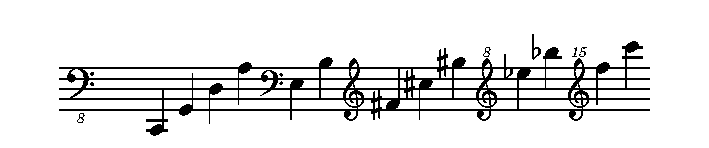
\includegraphics{examples/12-fifths.pdf}
\caption{The circle of twelve fifths}
\end{figure}
After proceeding through twelve fifths from our starting C, the final C is seven octaves
above it.
\begin{figure}[h]
\centering
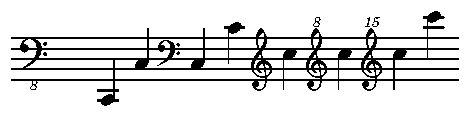
\includegraphics{examples/7-octaves.pdf}
\caption{The note C spanning seven octaves}
\end{figure}
If Pythagorean tuning was internally consistent, the C seven octaves above would be the
exact same pitch as the C resulting from twelve fifths.  We can test this mathematically,
by adding together twelve ratios of 3:2 and comparing them with the sum of seven octaves
using the ratio 2:1.\autocite[25]{RD:1}
\begin{equation}
    \frac{3}{2} \times
    \frac{3}{2} \times
    \frac{3}{2} \times
    \frac{3}{2} \times
    \frac{3}{2} \times
    \frac{3}{2} \times
    \frac{3}{2} \times
    \frac{3}{2} \times
    \frac{3}{2} \times
    \frac{3}{2} \times
    \frac{3}{2} \times
    \frac{3}{2} = \frac{531441}{4096} = 129.7463
\end{equation}
\begin{equation}
    \frac{2}{1} \times
    \frac{2}{1} \times
    \frac{2}{1} \times
    \frac{2}{1} \times
    \frac{2}{1} \times
    \frac{2}{1} = \frac{128}{1} = 128
\end{equation}
The mathematical result is that the sum of the twelve fifths is greater than the sum of
the seven octaves.  If we were to listen the these two pitches, they would not match.
The pitch resulting from twelve fifths above our starting C is noticeably sharper than 
the pitch resulting from seven octaves above the same starting note.

The additional problem with Pythagorean tuning was that it did not accurately reflect the
pitches in the harmonic series.
The first three pitches in the harmonic series matched Pythagorean ratios perfectly.  The
pure intervals of the octave, fifth and fourth in the harmonic series were exactly in tune
when compared to the ratios of their Pythagorean counterparts. However, the fourth pitch
in the harmonic series, the major third, when tuned acoustically pure as it naturally
occurred in the series, actually vibrated at a ratio of 5:4 and not 81:64, as the
Pythagoreans would have calculated by adding together two of their 9:8 wholetones: $ 9:8
\times 9:8 = 81:64 $.

These two tuning discrepancies that result from using only Pythagorean intervals to build
a scale of notes are called \textit{commas}.  The \textit{ditonic comma} results when
building a chromatic scale upon successive fifths, such as the difference between twelve
fifths and seven octaves, and the \textit{syntonic comma} results from the difference
between the pure harmonic 5:4 major third and the Pythagorean 81:64 major third.  The
Pythagoreans themselves were well aware of these problems and tried to overcome them, but
it was only Aristoxenus and Ptolemy who could offer a solution. Aristoxenus
proposal was to ignore the Pythagorean ideals of mathematical simplicity and use
tuning systems that divided the string according to parts and not ratios.  He described
tuning by using equal parts of the string and was the first to develop the concept of
tuning using equal semitones which would later be the foundation of equal temperament.
Ptolemy's proposal was to modify the Pythagorean notion of ratio by using only ratios that were
superparticular in nature, meaning that the first number of the ratio should always be one
unit great than the other.  So Pythagorean ratios like 2:1, 3:2, 3:4 and even 9:8 were
acceptable, but so too were other ratios such as 5:4, the pure major third, and 6:5, the
pure minor third.

Ptolemy's solution rectified a lot of the Pythagoreans' mathematical ratios with nature's
own internal tuning system but it still had problems when it came to musical execution.
In a twelve-tone scale, there are three major thirds. Starting on the note C, we can fit
three of them within an octave: C to E, E to G$\sharp$, and A$\flat$ to C.
\begin{figure}[h]
\centering
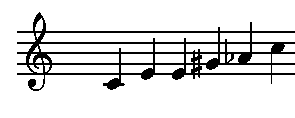
\includegraphics{examples/thirds.pdf}
\caption{Three major thirds within an octave}
\end{figure}
However, adding these intervals together using Ptolmey's ratios does not get us to a
complete octave either.  The sum of three thirds should sound the same as an octave with
the ratio 2:1, but the mathematical result is slightly less than 2, which sounds flat.
\begin{equation}
    \frac{5}{4} \times
    \frac{5}{4} \times
    \frac{5}{4} \times = \frac{125}{64} = 1.953125
\end{equation}
While the note E could remain fixed in relationship to the major third starting from C and
the major third ending on G$\sharp$, the fact that G$\sharp$ and A$\flat$ are used for the other
two major thirds implies that they are different notes. Most modern musicians regard the
enharmonic respelling of a note as a kind of music homonym: an alternative word to express
the same thing.  While the different names of G$\sharp$ and A$\flat$ can indicate different
functions, such as the third degree of the E major scale or the first degree of the A$\flat$
major, they are regarded today as notes having the same vibrating pitch. However, as
Ptolemy's tuning problem shows us, the two notes are not only functionally different, they
are musically different, and therefore tuned differently.

Ptolemy's solution of tuning with only pure intervals is known as just intonation.  While
it succeeded in correcting the problems associated with Pythagorean tuning, it made it
impossible to tune certain notes in the chromatic scale because they required a different
tuning according to the musical context in which they occurred.  Instruments of fixed pitches,
such as any keyboard instrument or fretted instrument, whose semitones were fixed and
immobile, could not accommodate a tuning of only pure intervals, or at least, not in a
scale of twelve tones.  Instruments of variable pitch, such as fretless bowed instruments,
wind instruments or the human voice were exempt from this problem because they were able
to adjust any note appropriately.  Violinists,
for example can place their fingers at any position along the fingerboard and wind players
who may vary the pitch of their notes using their embouchure.

What about Aristoxenus?  While he did invent an alternative solution of equal semitones,
he rejected both the notions of Pythagorean numeric purity and the Ptolemaic notion of
harmonic purity.  His method of tuning divided an octave into equal parts, creating
intervals as groups of these individual parts instead of using ratios at all.  His idea of
equal parts formed the basis for equal temperament.  While this allowed for a tuning of
fixed pitches in a chromatic scale, none of these intervals were tuned in a way that
precisely matched the tuning in the harmonic series.  This was an unacceptable solution
for most theorists and musicians during the evolution of western classical music, and it
took many years for equal temperament to gain acceptance.

Because the notion of equal semitones did not sit well with early western music theorists
and tuning harmonically pure intervals was impossible in a fixed pitch system, they
gravitated towards the Pythagorean system of tuning.  For one reason, it was simple,
using a small number of simple ratios.  For another, it matched
the musical tastes of the medieval period such as monophonic chants and polyphonic forms
based on fifths, unisons and octaves.  Pythagorean ratios persist even to this very day,
but as music changed in the early Renaissance period, composers sought to incorporate more
consonant thirds into their music, which the strict Pythagorean system of ratios did not
permit.  Thus, the old Greek debate between Pythagoras, Ptolemy and
Artistoxenus resurfaced.

\section{Temperament}

A temperament is a method of tuning a scale that alters an existing system, usually
Pythagorean tuning. For most of the Middle Ages, tuning was described according to the
ratios that Pythagoras had determined hundreds of years earlier. However, as musical
tastes changed during the Renaissance, there was an increasing preference for the sounds
of thirds instead of unisons and fifths. This represented the problem of rectifying thirds
within the Pythagoran tuning scheme that had plagued the Greeks centuries earlier. The
first attempts at a solution appeared at the end of the fifteenth century, and each one
took the same approach to solving the problem: changing the size of
the fifths within the existing Pythagorean system.

One of the first writers to publish a system that broke with the Pythagorean
tradition of tuning was Bartolomeus Ramis de Pareja.  In his \textit{Musica Practica} of
1482, he created a chromatic scale using two different groups of fifths.  Each group was
tuned in pure fifths, just as in Pythagorean tuning, except that one group was slightly
sharper than the other. \autocite[88]{MB:1}  Although he did not call it a temperament, it
technically was not Pythagorean tuning either.  Barbour credits Franchinus Gafurius's
\textit{Practica musica} of 1496 with the first mention of the idea of temperament.  In
it, Gafurius says that organists tune their fifths slightly flat, but does not go into any
specific details.\autocite[25]{MB:1} Similarly, Arnolt Schlick's 1511 treatise
\textit{Spiegel der Orgelmacher und Organisten} only gives us a general idea when he
refers to tuning the instrument's fifths flat, ``as much as the ear will permit.''
\autocite[202]{RR:1}  So while the idea was present as early as 1482, it took
several years for it to develop into a system.

Tempering is a process of compromise whereby the acoustical purity of one interval is
changed slightly in order to accommodate the acoustical impurity of another interval.
In this case, it is the process of changing the size of the fifth in order to
accommodate the major third which is not pure within the standard Pythagorean tuning.
This usually means shrinking the size of the fifth slightly so that it is narrower, or
flatter than the pure ratio of 3:2; although, in some cases a fifth may be tuned wider, or
sharper than pure. The problem with Pythagorean thirds were that they were much sharper
than pure, differing by the syntonic comma, which was the difference between the
Pythagorean third at 81:64 and the pure harmonic third at 5:4. Shrinking the size of the
fifth resulted in thirds that were flatter than the Pythagorean ratio of 81:54, closer to
the harmonically pure ratio of 5:4, and thus more appropriate sounding for music that
favored a greater number of thirds. Depending on how the fifth was flattened, you could
come very close to a pure 5:4 third, and the listener would not notice the
difference.  This was at the expense of the fifth, which was now flatter than pure but it
was an acceptable compromise because a flat fifth was less disconcerting than the
sharp third of Pythagorean tuning.  The strategy was to shrink several fifths by the same
or differing amounts. The result was that instead of one set of intervals being completely
pure and another unusable, all of the fifths were slightly
out-of-tune to differing degrees, while some of the thirds came very close to pure. Which
thirds approached pure and which fifths were made flat all depended on the particular
temperament, and there were many!

Murray Barbour classifies temperaments into four basic types: regular meantone, irregular
temperaments, equal division, and equal temperament. Whereas a tuning can be defined as a
method of obtaining intervals according to Pythagoras---as in Pythagorean tuning---or
according to Ptolemy---as in just intonation---temperaments alter the ratios of the
intervals so that they often lie somewhere between the two systems. In regular meantone
temperaments, most or all of the fifths in the Pythagorean tuning system are tuned flat by
the same amount.  Depending on which fifths are flattened, this can
result in thirds that are very close to pure; however, the fifths and fourths are not.  
The amount that each fifth was changed from its pure ratio often
depended on the musical context.  A meantone temperament with very flat fifths
resulted in a temperament with thirds quite close to pure, but because of the mutated
nature of the fifths, it was usable only in a limited number of keys.  Conversely, a
meantone temperament that tuned its fifths less flat made more keys playable, but resulted
in sharper, less pure thirds.

\subsection{Regular Meantone and Irregular Temperaments}

The first attempts at a systematic application of tempering fifths resulted in the class
of temperaments known as ``meantone.''  No one is entirely sure who invented the
first complete meantone temperament, but the general consensus is that it is a shared
prize between Pietro Aron and Gioseffo Zarlino. Zarlino is credited with the invention of an exact
system that narrows each fifth by $\frac{2}{7}$ of a syntonic comma.  His method, however,
was far from practical.  Although he provided a monochord diagram, his process of
tempering the fifths by that much actually created thirds that were smaller than pure, or
too flat.

Pietro Aron is credited with the first practical meantone temperament.  While not as theoretically
exact as Zarlino's, Aron's instructions can be used to create a workable meantone temperament that
narrows fifths enough to create pure thirds, while leaving the remainder of the intervals usable.
Unlike Zarlino, his instructions are not mathematical in nature require the person to tune by ear
and not rely on measurements.  His method was to start with pure thirds and build tempered fifths
around them.  He begins with a pure third between C and E and then proceeds to tune four fifths that
are all equally flat with additional pure thirds between A and C$\sharp$, and D and F$\sharp$.
While Aron says nothing about the division of the comma, Barbour takes these instructions and
mathematically proves that if the tuner is able to create Aron's pure thirds by ear and match the
size of the other fifths so that they are all tempered by the same amount, each of those fifths will
be flatter than pure by $ \frac{1}{4} $ of a syntonic comma.\autocite[27]{MB:1}  Because this is the
measurable amount that each fifth is reduced in size, Aron's temperament is referred to as
``quarter-comma meantone temperament.'' While Aron never referred to it this way, nor did he
mathematics to calculate lengths of a string, later theorists and musicians adopted his ideas and made
exact calculations that reproduced Aron's temperament.

Regular meantone temperaments contained eleven fifths that were all narrowed by the same
amount, measured as a fraction of the syntonic comma. Narrowing
four consecutive fifths in the circle of fifths by $ \frac{1}{4} $ of a syntonic comma was
enough to make eight thirds in a 12-tone scale pure while rendering the remaining four
unusable.\autocite[33]{RD:1}  This was an effective solution for
sixteenth-century music because it resulted in more serviceable keys than Pythagorean
tuning, and composers simply avoided the keys containing the unusable thirds.
This meant that meantone did not solve all of the problems associated with
Pythagorean tuning.  Just as Pythagorean tuning has a fifth that was too wide to be used,
meantone temperaments also had an unusable fifth.  The so-called ``wolf'' fifth existed in
every temperament, but its size and location depending on the kind of temperament.

As the sixteenth century continued, musicians attempted to correct the problems with
quarter-comma meantone, such as its wolf fifth and unusable thirds.
These tuning systems narrowed the fifth in smaller amounts, such as $
\frac{1}{5} $ or $ \frac{1}{6} $ of a syntonic comma. The result was that the thirds were
now sharper than pure but much less so than in Pythagorean tuning.  While this created
more usable thirds in the scale, the wolf fifth remained.  Sixth-comma meantone was
popular with fretted instruments, as we will see in a later chapter, but even sixth-comma
still contained the wolf fifth and unequal thirds.

The next major change in temperaments occurred in the seventeenth century when theorists began using
systems that narrowed fifths by varying amounts instead of equal amounts, as was the case with
regular meantone temperaments.  So called irregular temperaments, or well temperaments, became very
popular and widespread in the seventeenth and eighteenth centuries.  The advantage of well
temperaments was that musicians had finer control over which intervals were problematic.  For
example, in quarter-comma meantone, the fifth between E$\flat$ and A$\flat$ will always be too wide
to be used.  Technically, this is because the A$\flat$ is really a G$\sharp$. \autocite[35]{RD:1}
Similarly, the thirds B to D$\sharp$, D$\flat$ to F and F$\sharp$ to A$\sharp$ would also be
unacceptable.  With irregular temperaments, fifths were narrowed by differing amounts so that the
wolf fifth was eliminated, and normally problematic thirds in standard quarter-comma meantone could
be made more tolerable by adjusting the size of other intervals instead. These irregular
temperaments were similar to regular meantone temperament, except that one fifth might be narrowed
one-quarter of a comma, while another might be narrowed only by a sixth or less.  As a result, the
composer had more control over which keys had better-sounding thirds and which did not.

The introduction of irregular temperaments caused an explosion in the number and variety of
temperaments available to musicians in the seventeenth and eighteenth centuries. Theorists such as
Valloti, Young, Werckmeister and others all developed their own systems of temperament favoring
different intervals in ways that regular meantone temperaments could not.  Composers also developed
their own temperaments as well, such as J. S. Bach who used his own temperaments in the performance
of his keyboard works.  His compositions in \textit{The Well-Tempered Clavier} were so named because
of the temperament he used for them that allowed use of all keys on the instrument.

\subsection{Equal Division}

All of the methods described thus far are practical ways to create temperaments.
For example, Aaron's method uses the ear alone and produces a good quarter-comma 
meantone temperament without the need for complex mathematical calculations. Later methods
of tuning other meantone temperaments and well temperaments used the same techniques of
narrowing or widening intervals by certain amounts, either by ear or by some process of
calculation.

The problem with some of these methods is that they are imprecise. The
fifth is narrowed by an indeterminate amount to match a pure third or
intervals are determined by counting the number of beats that occur as pitches
essentially clash against one another.  Most importantly, the resulting temperaments
contain semitones that vary in size according to the placement of the tempered intervals.
If we are to compare different temperaments and their specific pitches, we need a more
exact way of calculating a given pitch in a given temperament.

Recalling Aristoxenus in our survey of Greek tuning methods, his approach consisted of
dividing a string or octave into equal parts and creating intervals by grouping tones into
sets of these equal parts. Using this same method, we can create several different regular
meantone temperaments by dividing our octave into multiple parts and combining
wholetones and semitones into a groups. The advantage to using this method as
opposed to other methods like Aaron's, is that we can compare semitone sizes more
accurately across different kinds of temperaments and we may also quantify the difference
in the sizes of our semitones. Barbour refers to this process of calculating temperaments
as equal division. Equal division was used in the sixteenth century to calculate string
lengths for both quarter and sixth comma meantone temperaments, and its principles
remained in use well into the seventeenth and eighteenth centuries.

The first theorist to use equal division was Vicentino in 1555, who divided his octave
into 31 parts using a harpsichord that contained six ranks of keys. Vicentino was
attempting to create a temperament like quarter-comma meantone, but instead used the
principles of equal division instead of Aron's tempered fifths. In order to create an
octave of 12 tones out of a total of 31 parts, he combined five parts in each wholetone
and made semitones of two different sizes, a smaller semitone with two
parts and a larger semitone with three.  The size of the semitone depended on where it
occurred within the scale. Musicians during the sixteenth and seventeenth centuries
were familiar with these differences in semitone size and referred to the larger
semitone as the \textit{major semitone} and the smaller semitone as the \textit{minor
semitone}.  The difference in size between the two semitones was referred to as a
comma.  We should not confuse this with the diatonic or syntonic comma, which are
differences of pitch as well but have no correlation in systems of equal division.

Vicentino's 31-part system solved the same kinds of problems that meantone temperament
did, namely that of creating pure thirds at the expense of pure fifths. However, it had
the added advantage of clearly indicating that semitones differed in size by one comma.
Other approaches to meantone temperament, such as Aaron's, were less specific and would
tune certain semitones to a midway point between the wholetone it was dividing.  This
was usually reserved for the wolf fifth or the chromatic notes which were less likely
to be used.  As musicians developed systems of equal division, they utilized keyboards
that could realize the distinction between semitones more accurately and used split
keys that enabled one to play either diatonic or chromatic semitones.  The use of
enharmonic instruments that had more than twelve notes per octave dates back to the
late fifteenth century, and Patrizio Barbieri's recent book documents them
extensively.\autocite{PB:1} Vicentino's multi-manual keyboard was one example of such
an instrument, but was too impractical to use. More practical examples of keyboards
with split keys were found later in the seventeenth century, especially in Italy. These
instruments had different keys for some or all of the accidentals; composers and keyboardists
such as Handel and Werkmeister continued to use them into the eighteenth century.
\autocite[108]{MB:1}

Examining the 31-part system in more detail, let us take the C major scale as an example containing
five wholetones: C, D, F, G, A; and two semitones: E and B. In our system, we reach 31 parts by
assigning 5 parts to each wholetone and 3 parts to each semitone in the scale.  
Figure~\ref{31-part-octave} shows the arrangement of each pitch in the scale according to its number of parts.
% 31 division octave
\begin{figure}[h]
\centering
\setlength{\unitlength}{1mm}
\begin{picture}(96, 30)
  %\put(0,0){\circle*{1}}
  %\put(96,0){\circle*{1}}
  %\put(0,30){\circle*{1}}
  %\put(96,30){\circle*{1}}
  \linethickness{.075mm}
  \multiput(2, 15)(3, 0){32}{\line(0, 1){4}}
  \linethickness{.5mm}
  % C
  \put(2,12){\line(0,1){9}}
  \put(0,24){$C$}
  % D
  \put(17,12){\line(0,1){9}}
  \put(15,24){$D$}
  % E
  \put(32,12){\line(0,1){9}}
  \put(30,24){$E$}
  % F
  \put(41,12){\line(0,1){9}}
  \put(39,24){$F$}
  % G
  \put(56,12){\line(0,1){9}}
  \put(54,24){$G$}
  % A
  \put(71,12){\line(0,1){9}}
  \put(69,24){$A$}
  % B
  \put(86,12){\line(0,1){9}}
  \put(84,24){$B$}
  % C
  \put(95,12){\line(0,1){9}}
  \put(93,24){$C$}
\end{picture}
\caption{The C major scale in a 31-part system}
\label{31-part-octave}
\end{figure} 
Five wholetones at 5 parts apiece makes 25 parts, and adding
the remaining semitones at 3 parts each gives us a total of 31: $ 25 + 3 + 3 = 31 $. Note that
semitones E to F and B to C have 3 parts as opposed to 2.  As we divide our scale further into
chromatic pitches, each wholetone is divided into 2 and 3 parts.  Semitones that are diatonic within
a scale, such as E and B in a C major scale, always contain 3 parts as opposed to 2. The smaller
semitone is reserved for chromatic notes that lie outside the scale. For this reason, the larger
semitone is sometimes referred to as the \textit{diatonic semitone} while the smaller of the two is
called the \textit{chromatic semitone}. Figure~\ref{31-part-octave-complete} shows the rest of our C
major scale divided into its chromatic and diatonic semitones. 
% 31 division octave
\begin{figure}[h]
\centering
\setlength{\unitlength}{1mm}
\begin{picture}(96, 30)
  %\put(0,0){\circle*{1}}
  %\put(96,0){\circle*{1}}
  %\put(0,30){\circle*{1}}
  %\put(96,30){\circle*{1}}
  \linethickness{.075mm}
  \multiput(2, 15)(3, 0){32}{\line(0, 1){4}}
  \linethickness{.5mm}
  % C
  \put(2,12){\line(0,1){9}}
  \put(0,24){$C$}
  % C#
  \put(8,14){\line(0,1){7}}
  \put(7,24){$C\sharp$}
  % Db
  \put(11,12){\line(0,1){7}}
  \put(9,7){$D\flat$}
  % D
  \put(17,12){\line(0,1){9}}
  \put(15,24){$D$}
  % D#
  \put(23,14){\line(0,1){7}}
  \put(22,24){$D\sharp$}
  % Eb
  \put(26,12){\line(0,1){7}}
  \put(24,7){$E\flat$}
  % E
  \put(32,12){\line(0,1){9}}
  \put(30,24){$E$}
  % F
  \put(41,12){\line(0,1){9}}
  \put(39,24){$F$}
  % F#
  \put(47,14){\line(0,1){7}}
  \put(45,24){$F\sharp$}
  % Gb
  \put(50,12){\line(0,1){7}}
  \put(48,7){$G\flat$}
  % G
  \put(56,12){\line(0,1){9}}
  \put(54,24){$G$}
  % G#
  \put(62,14){\line(0,1){7}}
  \put(60,24){$G\sharp$}
  % Ab
  \put(65,12){\line(0,1){7}}
  \put(63,7){$A\flat$}
  % A
  \put(71,12){\line(0,1){9}}
  \put(69,24){$A$}
  % A#
  \put(77,14){\line(0,1){7}}
  \put(75,24){$A\sharp$}
  % Bb
  \put(80,12){\line(0,1){7}}
  \put(78,7){$B\flat$}
  % B
  \put(86,12){\line(0,1){9}}
  \put(84,24){$B$}
  % C
  \put(95,12){\line(0,1){9}}
  \put(93,24){$C$}
\end{picture}
\caption{The chromatic scale in a 31-part system}
\label{31-part-octave-complete}
\end{figure} 
Chromatic semitones represent the shortest distance between two pitches, such as the
distance from C to C$\sharp$, but this is also the same distance as G descending to G$\flat$.
Likewise, the distance ascending from C to D$\flat$ is the larger, diatonic semitone as well as the
descending distance from G to F$\sharp$. The term diatonic semitone might be misleading since it
implies that D$\flat$ or F$\sharp$ are diatonic to a C major scale.  For this reason, the minor and
major designations are preferable.

Systems of equal division were not limited to just 31 parts.  Zarlino and Salinas
describe a 19-division octave in the sixteenth century, and later systems included
octaves divided into 43 and 55 parts.  Each of these systems grouped their wholetones
into an odd number of parts and therefore had their semitones divided unequally with a
comma's different between them. Praetorius, in his \textit{Syntagma Musicum}, describes
a 55-part system with nine parts per wholetone and semitones of four or five parts.  He
describes this system in reference to the ``intermediate'' nature of the semitones on
fretted instruments:
\begin{blocks}
Thus the semitones cannot be either major nor minor, but are, perforce, ``intermediate''
if anything. For I reckon that each fret [...] contains four-and-a-half commas, whereas
the major semitone contains five and the minor semitone only four. Since the error is
only half a comma either way, the ear hardly notices it with these instruments [...]
Major and minor semitones are both produced by the same fret, both sound in tune, [...]
especially since by particular applications of the finger to the string, over the fret,
it is possible to have some control over the pitch of the note produced.
\autocite[68]{MP:1}
\end{blocks}
As late as 1723, singer and teacher Pier Francesco Tosi expressed the same idea, though
not in reference to fretted instruments, in his treatise \textit{Opinioni de Cantori}:
\begin{blocks}
A Tone, that gradually passes to another, is divided into nine almost imperceptible
Intervals, which are called Comma's, five of which constitute the Semitone Major, and four
the Minor.
\autocite[20]{PFT:1}
\end{blocks}
Praetorius and Tosi are both describing a system of equal division.  Tosi was writing in
the eighteenth century, but equal division as a tuning method had already been in use
since the sixteenth century when it was used to mimic the same features of quarter-comma
meantone.

The basic features of each of these systems is outlined in table
~\ref{table:equalDivision}, where the corresponding meantone temperament is given.  Of
the four that are listed, quarter-comma and sixth-comma are the most significant
because they were the most frequently used of the meantone systems.
\begin{table}[h!]
  \begin{center}
  \scalebox{0.7}
  {
    \begin{tabular}{ c c c c c}
      Number of Divisions & Wholetone & Major semitone & Minor semitone & Meantone equivalent \\
      \hline
      19 & 3 & 2 & 1 & third-comma meantone \\
      31 & 5 & 3 & 2 & quarter-comma meantone \\
      43 & 7 & 4 & 3 & fifth-comma meantone \\
      55 & 9 & 5 & 4 & sixth-comma meantone \\
      67 & 11 & 6 & 5 & seventh-comma meantone \\
      79 & 13 & 7 & 6 & eighth-comma meantone \\
    \end{tabular}
  }
  \end{center}
  \caption{Comparison of systems of equal division}
  \label{table:equalDivision}
\end{table}
Quarter comma was used almost exclusively by keyboard and wind instruments, and was the
same kind of temperament that Vicentino was advocating with his system. Sixth-comma turns
out to be the same temperament that Praetorius, and later Tosi, were describing although
neither refer to it by that name.  I will return to Praetorius's observation about
sixth-comma temperament when we examine other specific temperaments for fretted
instruments later.

Although they each have different parts, each of the above systems function the same way
as Vicentino's original 31-division octave. In a 19-division octave, whole tones consist
of three parts, and major and minor semitones are two and one parts respectively.  43-part
systems contain whole tones with seven parts each, dividing their semitones between four
and three parts, and then a 55-part system has nine parts for its whole tones, divided
into five and four.  Other systems were possible that created seventh and eighth comma
meantone; however, these were not used to any great extent since their tunings began to
approximate equal temperament and from a practical standpoint, did not serve as good a
purpose.

\subsection{Equal Temperament}

Technically speaking, equal temperament is a type of division in which the octave is
divided into twelve equal parts.  In terms of its qualities as a temperament, it
compensates for the ditonic comma the same way a meantone temperament does by narrowing
the fifth. The difference between equal temperament and meantone temperament is that
meantone will narrow its fifths much more than equal temperament.  In equal
temperament, all twelve fifths of the scale are narrowed by a slight but equal amount.
The ditonic comma is therefore dispersed throughout the entire scale so that every
pitch is usable, but this ability has its price.  The temperament creates thirds that
are as sharp as they possibly can be without having too strong an effect on the
listener.  While they are not as sharp as the thirds of Pythagorean tuning, they lack
the pure quality of a quarter-comma meantone temperament and are too sharp to
approximate it in the way that other meantone and irregular temperaments do. However,
the homogeneous nature of every third being sharp by the same amount tends to veil this
lack of harmonic purity from our ears, so that it is not as noticeable.

Even with its overly sharp thirds, theorists in the sixteenth century regarded equal
temperament as a technical impossibility. Because everyone based their tunings on the
Pythagorean 9:8 wholetone, it was mathematically impossible to divide it into two
geometrically equal, whole-number ratios. They could only divide the whole tone
unequally into a larger semitone of 17:16 and a smaller one of 18:17.
\autocite[20]{ML:1} If we recall that adding two geometrical ratios together requires a
process of multiplication, then when 18:17 and 17:16 are ``geometrically'' added
together, it produces the 9:8 ratio.
\begin{equation}
  \frac{18}{17} \times
  \frac{17}{16} =
  \frac{306}{272} =
  \frac{\frac{306}{34}}{\frac{272}{34}} =
  \frac{9}{8}
\end{equation}
The difference between the two ratios is similar to the same differences in semitone size
found in meantone temperaments and systems of equal division.  The smaller 18:17 ratio is
the minor semitone and the larger 17:16 ratio is major semitone.

Although equal temperament was impossible according to geometry, musicians knew
how to approximate it very closely without having to worry about the mathematics.
Despite this ability, almost everyone preferred meantone temperaments because of
their pure thirds. Even later in the seventeenth and eighteenth centuries,
irregular temperaments were still favored over equal temperament because they
made more keys feasible and were able to produce some thirds that were much
closer to pure than their equally-tempered counterparts.

A tuning method very similar to equal temperament appeared in Giovanni Maria
Lanfranco's \textit{Monocordi \& Organi} of 1533.  His system does not attempt to
divide the octave into twelve parts, but instead mimics the quality of the fifth found
in systems that do.  He describes a system where the fifths are tuned slightly flat and
the thirds are made as sharp as the ear can possibly endure. \autocite[45]{MB:1} Other
writers after him described the same kind of system, sometimes giving him credit and
sometimes not.  Although Lanfranco's temperament made it possible to use more pitches
of the chromatic scale, just as equal temperament does, it still created overly sharp
thirds making it inferior to meantone temperament at the time.

One of the first systems to create equal temperament using measurable means was known
as the \textit{18:17 rule}. The theorist and lute player Vincenzo Galilei is credited
with developing it for practical use. \autocite[57]{MB:1}  Although technically not
true equal temperament, Galilei created twelve semitones of the same size in an octave
using a series of Pythagorean minor semitones, or the smaller ratio of the 9:8
wholetone, the 18:17 semitone.  His procedure was relatively straightforward:  A string
is divided into 18 equal parts, and the first part or $ \frac{1}{18} $ of the string,
is marked as the first semitone.  The remaining length or $ \frac{17}{18} $ of the
string is then redivided into another 18 different parts.  The first part of this
division is then marked as the second semitone.  The process is then repeated with the
remaining string length to mark the third semitone, and so on, each time redividing the
remaining amount of string into 18 parts and marking the first part as the next
semitone.

Since the Pythagorean minor semitone is slightly smaller than an equally tempered
semitone, Galilei's system was not the same as modern equal temperament, but was a way
to divide the octave into twelve useable semitones. Since each successive semitone is a
bit flat, the fifth is slightly flat as well, very close to an equally-tempered fifth
with the octave flat as well and not pure.  This issue seemed to go unnoticed on
fretted instruments because of the way in which pitches  tend to be sharper at
higher frets.  Since Galilei was a lutenist, he was using temperaments that he found
the best for his instruments.  While this worked well for the lute, it did not
apply to non-fretted instruments.  The same feature of sharp thirds
still remained in Galilei's method just as it did with all other temperaments at this
time that approximated equal temperament.

Despite the predominance of meantone temperament in the sixteenth century, many shared
Galilei's opinions and accepted the fact that lutes and other fretted instruments should
be tuned with equal semitones.  These included such notable musicians as Vicentino,
Zarlino, Salinas, Artusi, Praetorius and Mersenne. \autocite[19]{ML:1} This did not
mean that lutes were tuned in the same kind of equal temperament that we find today. As
we will see later, there were variations in which lutes and other fretted
instruments approximated equal frets as well as making their frets unequal to match
common meantone temperaments.

Equal temperament was not fully accepted in musical practice until at least the
eighteenth century, and even as late as the twentieth.  Ross Duffin provides ample
evidence that musicians were tuning their fifths flatter than those in today's equal
temperament systems well into the nineteenth century, and that true equal temperament
really did not become a indisputable fact until 1917 when it was standardized.
\autocite[138]{RD:1}  After that, the advent of modern electronic tuning devices that
enabled tuners and musicians to calculate a correctly tempered fifth precisely,
solidified equal temperament's place in the modern musical world.

\section{Describing Temperaments}

Throughout the course of this study, we will need to refer to the qualities of the different
temperaments explained thus far as well as compare them to other lute-specific temperaments that we
will encounter in later chapters.  Audio examples can illustrate the differences between
temperaments, but sometimes they are so slight that even the most trained ear might have difficulty
in distinguishing them, or be unable to describe the difference accurately. For example, it might be
difficult for any of us to distinguish between a fifth that had been narrowed by one fifth of a
comma versus one that was narrowed by a sixth.  Furthermore, comparing several different
temperaments with audio examples in the context of a written paper can impede the reader, and
papers, of course, do not have speakers built into them.

Expressing temperaments using numerical means is one of the best means of pinpointing the exact
difference between intervals in a written environment, and we can do this in several different ways.
The first, which I have already used, describes intervals as whole-number ratios, as the Greeks did
thousands of years ago.  This was also the way that most others employed in the sixteenth and
seventeenth century as well, including lutenists.  For that reason, I will use these whole-number
ratios whenever possible to refer to numerical differences between intervals. However, not all
intervals are easily defined using these kinds of ratios.

Meantone temperament uses intervals that can be expressed as whole number ratios,
but these are not easily derived.  We can calculate the ratios of meantone intervals in
two ways: The first involves determining the parts of a comma and subtracting them
from the fifth, as Aaron originally suggested.  The only difference is that Aaron
was using his ear to achieve this, but here we will propose a more rigorous arithmetical
method to achieve the same result.  Furthermore, we shall also need to
precisely articulate the differences of semitone and interval size in a variety of
meantone temperaments.

Because each system of meantone temperament has a matching system of equal
division, we can express its intervals mathematically with the same system of parts or
commas that were used historically.  For example, in Vicentino's 31-part octave, the fifth
would comprise three whole tones and a major semitone. Referring to
figure~\ref{31-part-octave}, that makes a total of 18 parts out of the total 31.  We
can represent this mathematically using the ratio of parts as a logarithmic function:
$2^\frac{18}{31}$.  Applying the same ratios of parts as exponential fractions, we can
calculate any interval in any meantone system, such as the quarter-comma major
semitone: $ 2^\frac{3}{31} $; or the sixth-comma major semitone: $ 2^\frac{5}{55} $.
Incidentally, we can also express intervals in equal temperament the same way.  For
example, the semitone in equal temperament is: $ 2^\frac{1}{12} $; the whole tone $
2^\frac{2}{12} $; the fifth: $ 2^\frac{5}{12} $ and so on.  The obvious problem with these numeric
representations is that are more difficult to comprehend than a simple number, and are
not readily comparable to standard Pythagorean ratios.

In order to compare all these different kinds of semitones effectively, we need to
express either their ratio or their logarithmic formula as a simple decimal number. In
this case, the number could be applied to a string length to determine what length of
string would produce a sixth-comma meantone major semitone, a quarter-comma meantone
fifth or pure third, and it can also determine the vibrating frequency for those
particular pitches as well. Referring to table~\ref{fifth-comparison}, if we compare
the Pythagorean ratio 3:2 with its quarter-comma meantone equivalent, expressed using
logarithmic functions, we can immediately see that the Pythagorean fifth is slightly
larger.  We also see that the the quarter-comma third matches the ratio of the
pure third more closely, as opposed to the fifth or sixth-comma third.
\begin{table}[h!]
    \begin{center}
    \begin{tabular}{ r l }
        Pythagorean fifth:            & $ 3:2 = 1.500 $ \\
        Quarter-comma meantone fifth: & $ 2^\frac{18}{31} = 1.4955 $ \\
        \hline
        Pure third:                   & $ 5:4 = 1.2500 $ \\
        Third-comma meantone third:   & $ 2^\frac{6}{19} = 1.2447 $ \\
        Quarter-comma meantone third: & $ 2^\frac{10}{31} = 1.2506 $ \\
        Fifth-comma meantone third:   & $ 2^\frac{14}{43} = 1.2532 $ \\
        Sixth-comma meantone third:   & $ 2^\frac{18}{55} = 1.2546 $ \\
    \end{tabular}
    \end{center}
    \caption{Comparison of pure and meantone fifths and thirds using decimal equivalents}
    \label{fifth-comparison}
\end{table}
We know from Aaron's description of tuning meantone temperament that the fifth was
tuned slightly flatter than pure, and the chart also bears this out, with the
quarter-comma fifth smaller than the pure fifth.

The decimal equivalents I am choosing to use to express these differences do not
have any musical significance. However, the useful feature of these simple decimal
numbers is that one can easily rank the different temperaments from smaller to larger,
or flatter to sharper. Larger numbers indicate a larger or wider interval that is
sharp.  Conversely, smaller numbers indicate smaller or narrower intervals that are
flat.  With the ability to calculate any kind of semitone, whether chromatic or
diatonic, in any meantone temperament quarter-comma or otherwise, we can now correctly
determine what kind of temperament and semitones lute fretting systems used.  That is
the matter to which we now turn directly.